\section{Analysis of the Experiment}
\label{sec:Auswertung}



\subsection{LED to Laserdiode}
\label{sec:LED_Laser}
First a threshold current of
\begin{align}
I_{\mathrm{threshold}} = \SI{33,7}{\milli\ampere}
\end{align}
is measured.
Furthermore in figure \ref{fig:threshold} the two
pictures from the camera focusing on the card are shown.
With the difference, that on one picture the current of the diode is below threshold \ref{fig:LED} and
on the other it is above threshold \ref{fig:LASER}.
\begin{figure}
  \centering
  \begin{subfigure}{0.45\textwidth}
    \centering
    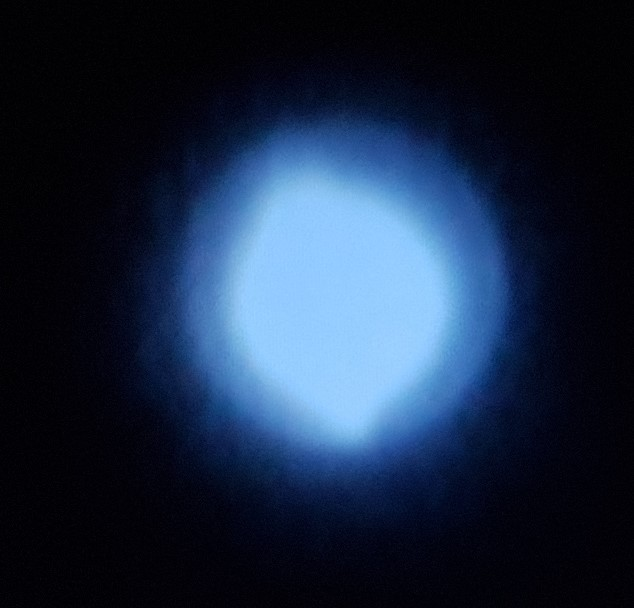
\includegraphics[height = 5cm]{figures/bevore_threshole.jpg}
    \caption{LED}
    \label{fig:LED}
  \end{subfigure}
  \begin{subfigure}{0.45\textwidth}
    \centering
    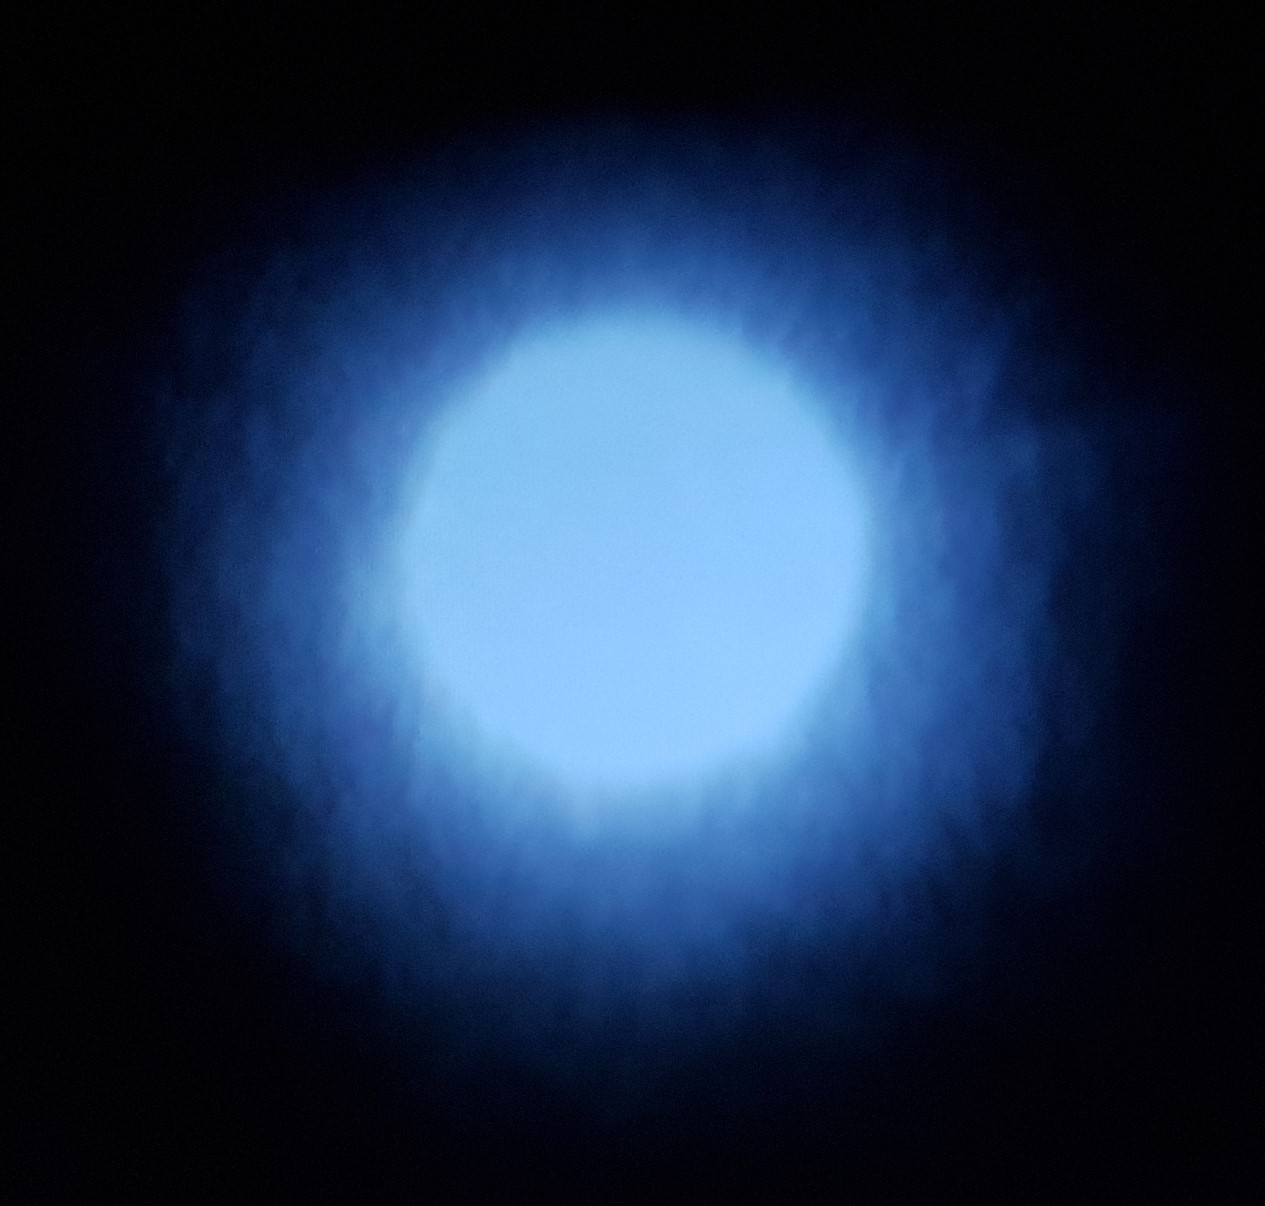
\includegraphics[height = 5cm]{figures/after_threshole.jpg}
    \caption{LASER}
    \label{fig:LASER}
  \end{subfigure}
\caption{The light below \ref{fig:LED} and above \ref{fig:LASER} the current threshold.}
\label{fig:threshold}
\end{figure}
The intensity change of the diode beam is clearly recognizable
between the lower intensity LED radiation \ref{fig:LED}
and the higher LASER radiation\ref{fig:LASER}.
% so the theory of a threshold current can be confirmed.


\subsection{Rubidium fluorescence}
\label{subsec:RB_fluorescence}

It follows the results for the setup \ref{fig:setup2}.
First with the rubidium absorption cell located in the laser beam
and the current adjusted, so rubidium fluorescence is observed. The picture of the
camera, which is targeted at the
rubidium absorption cell, is
displayed in the figure \ref{fig:fluores}.

\begin{figure}
  \centering
  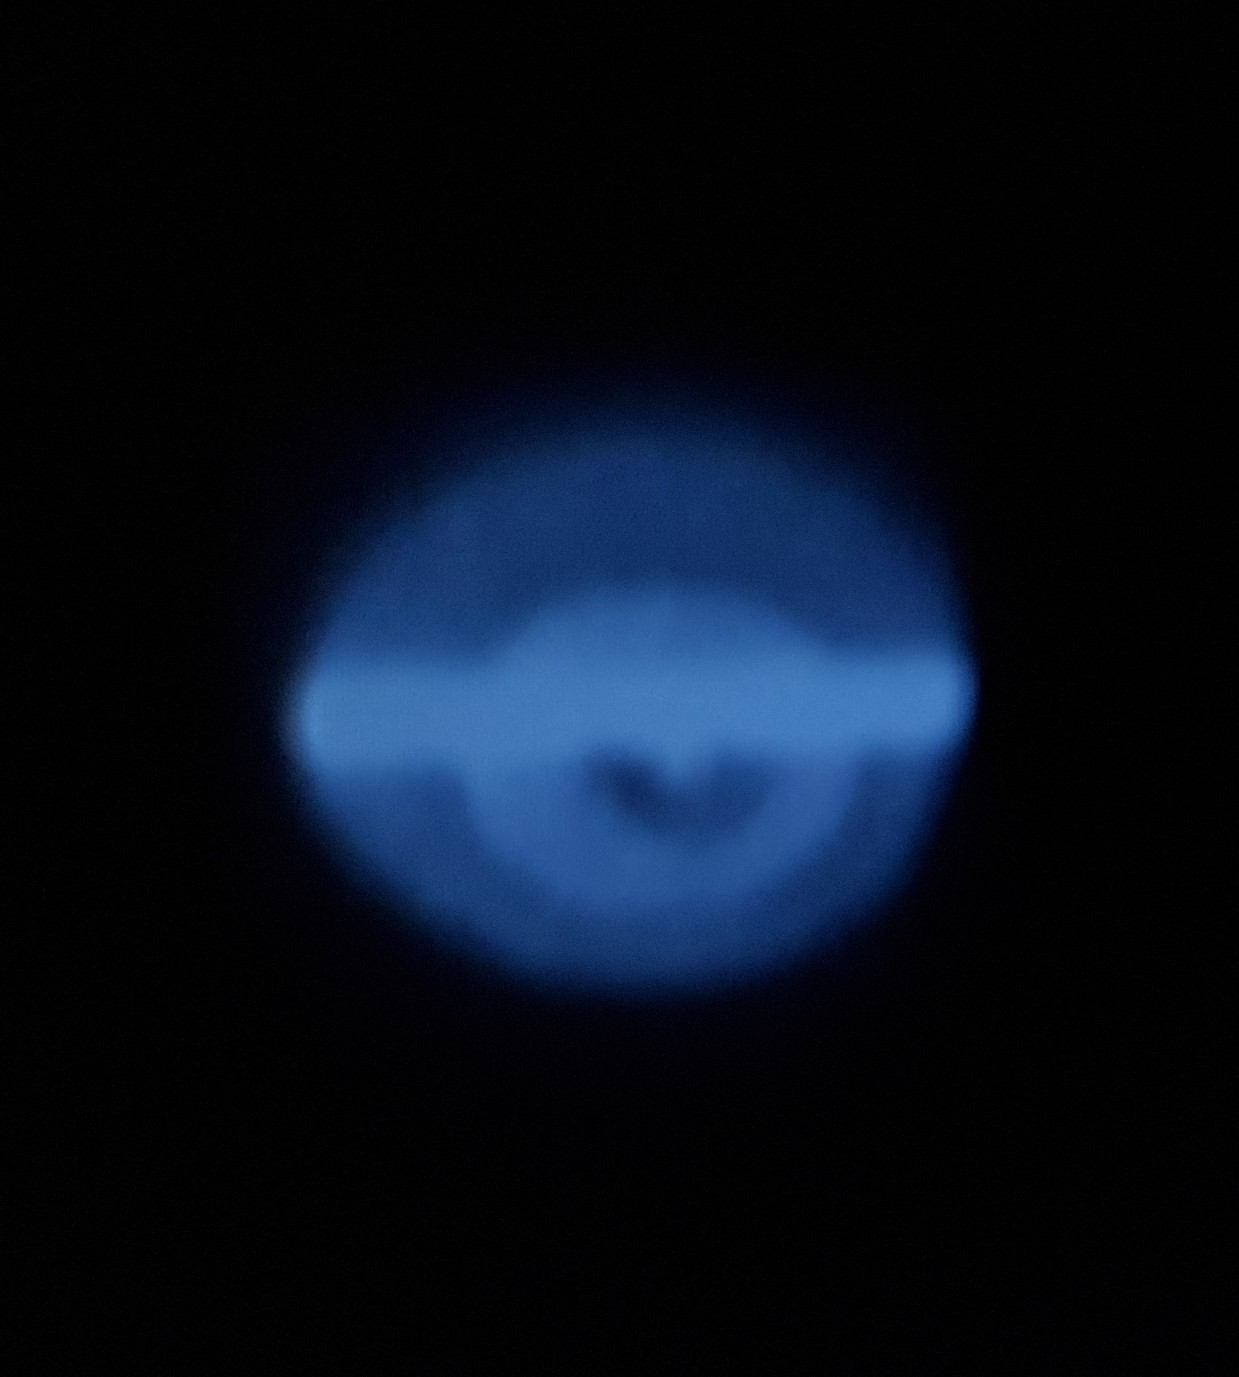
\includegraphics[height = 6cm]{figures/Rb_leuchten.jpg}
  \caption{Observation of the rubidium fluorescence.}
  \label{fig:fluores}
\end{figure}

Rubidium fluorescence is only observed along the laser beam, therefore
the brighter horizontal line
in figure \ref{fig:fluores}
is the track of the laser beam
going through the rubidium cell and stimulating the rubidium atoms.


\subsection{Rubidium absorption spectrum}
\label{subsec:Rubidium_absorptionspectrum}


Now with the active ramp generator moving the grating with the piezo stack,
the signal from the photodiode behind the rubidium cell
is displayed with an oscilloscope and shown in figure \ref{fig:ramp}.
Also the signal of the ramp generator is shown in the same
figure.

\FloatBarrier
\begin{figure}
  \centering
  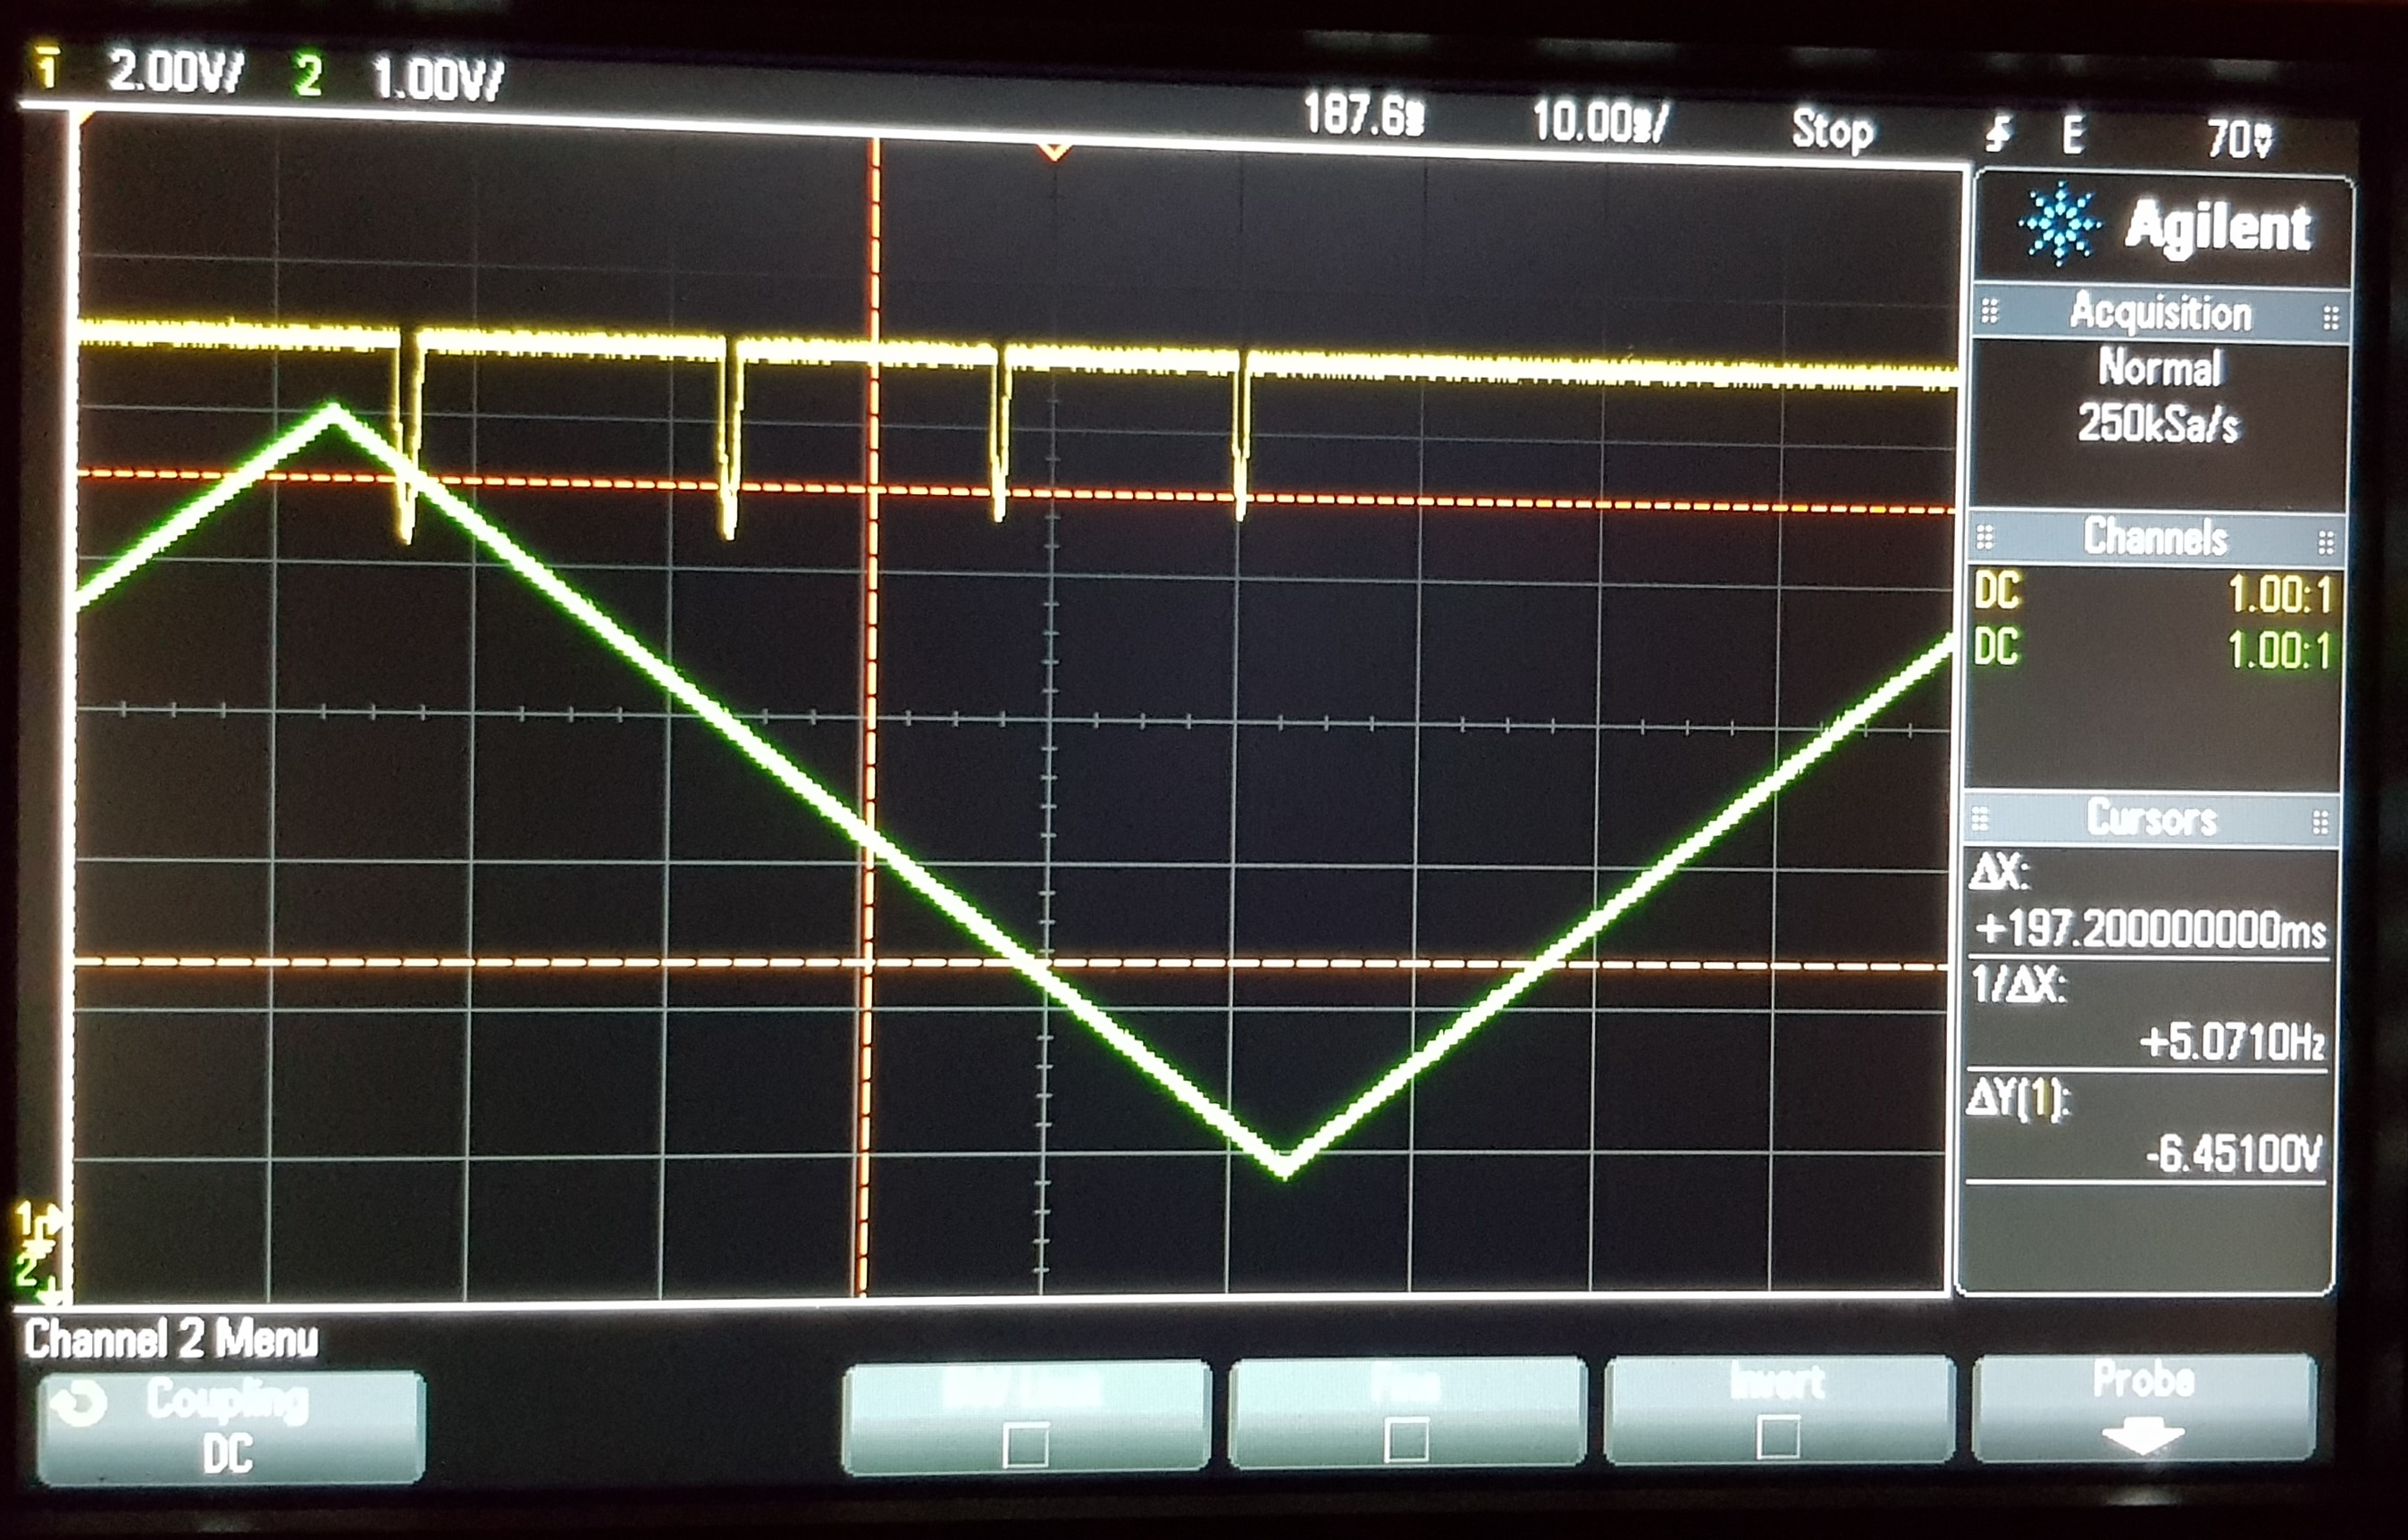
\includegraphics[width = 0.7\textwidth]{figures/Ramp.jpg}
  \caption{Signal from the photodiode and the ramp generator.}
  \label{fig:ramp}
\end{figure}
\FloatBarrier

The figure \ref{fig:ramp} contains a part of the
absorption spectrum as required.
Due to a problem with the storage device, the pictures of the remaining
measurements, where only one photodiode is used, are lost.
Nevertheless an image of the hole rubidium spectrum
with a simultaneous current and piezo modulation
can be produced. To get an impression of the possible image,
in figure \ref{fig:theory_curve} an example is displayed.

\FloatBarrier
\begin{figure}
  \centering
  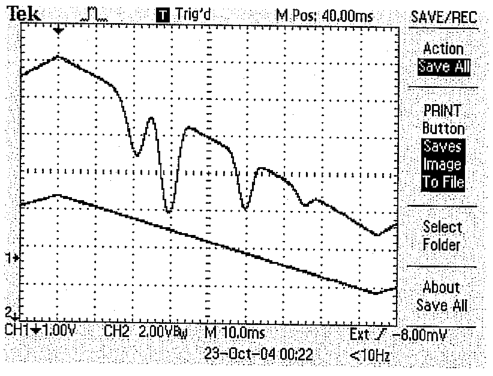
\includegraphics[width = 0.5\textwidth]{Rb_modulation.png}
  \caption{Signal from the photodiode and the ramp generator with
  simultaneous current and piezo modulation. \cite{V60}}
  \label{fig:theory_curve}
\end{figure}
\FloatBarrier

Fortunately an oscilloscope image of the second measurement
with two Photodiodes
is available and displayed in figure \ref{fig:2dioden}.

\FloatBarrier
\begin{figure}
  \centering
  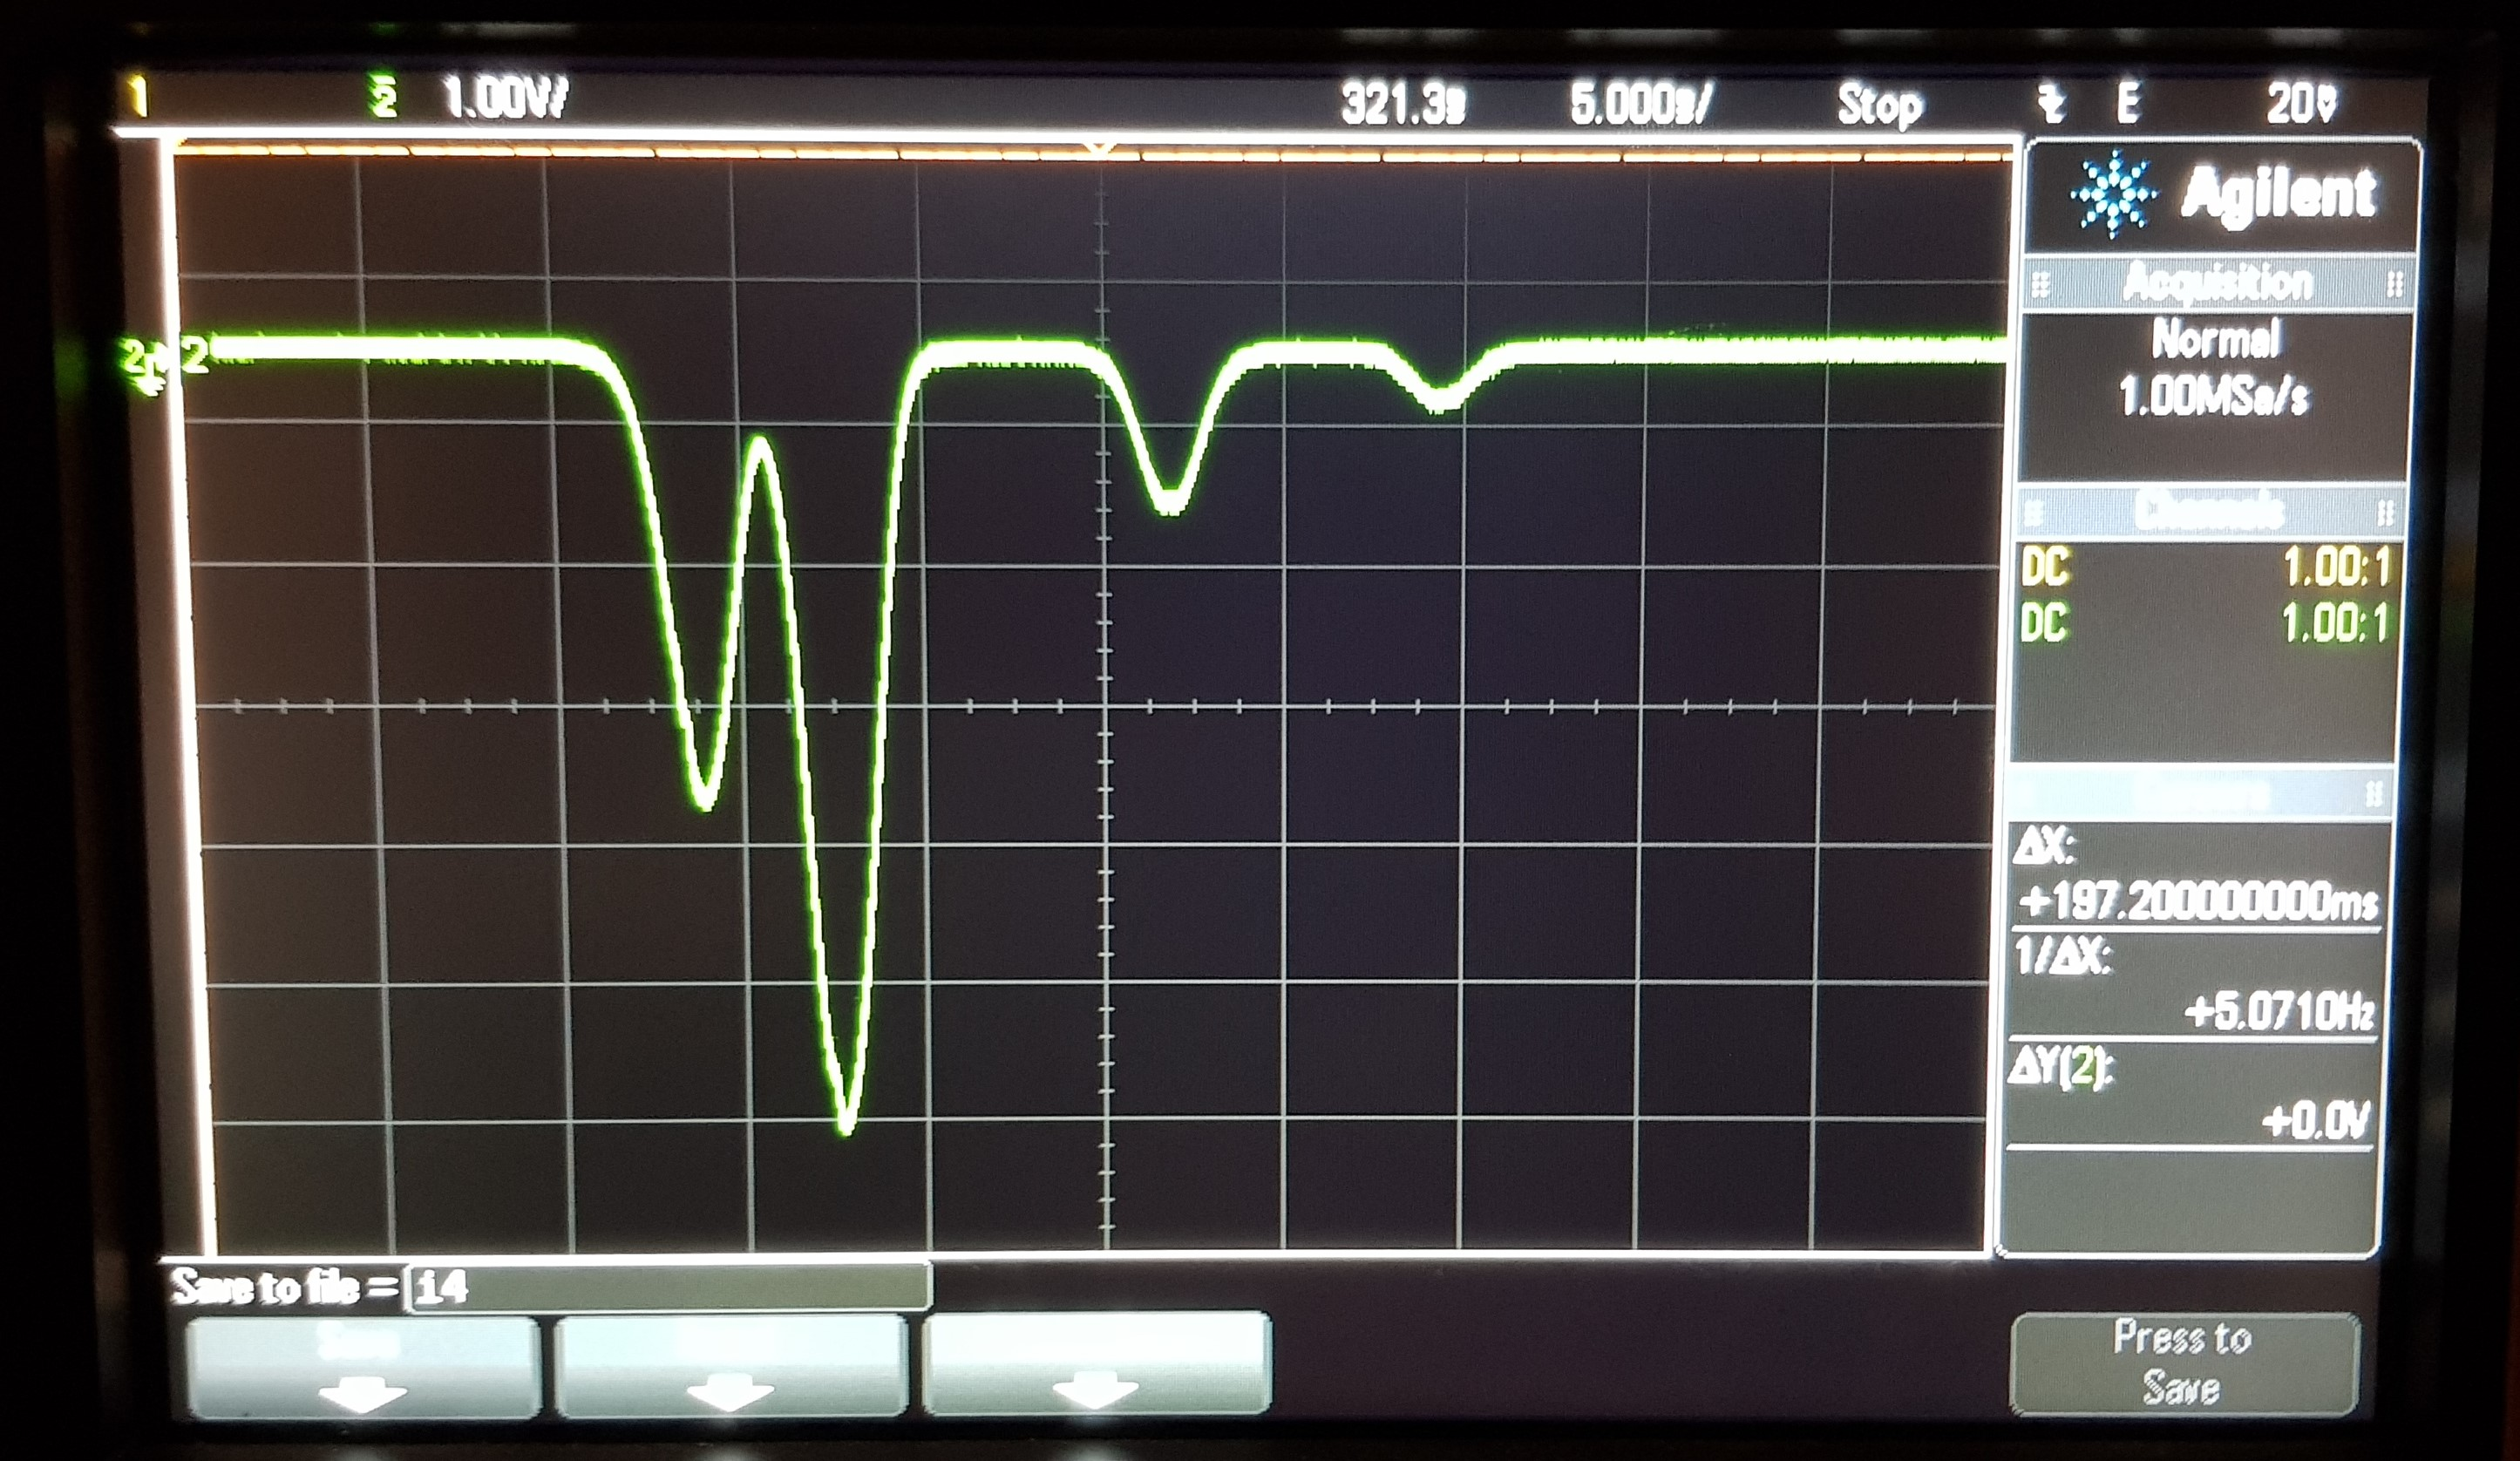
\includegraphics[width = 0.7\textwidth]{./figures/Rb_spectrum.jpg}
  \caption{Mixed signal from the two photodiodes and active ramp generator with
  simultaneous current and piezo modulation.}
  \label{fig:2dioden}
\end{figure}
\FloatBarrier

In contrast to the signal in figure \ref{fig:theory_curve}
the signal in figure \ref{fig:2dioden} the
ramp generator signal is not contained in the mix signal anymore.
